\subsection{BBC Recipes}

\begin{figure}
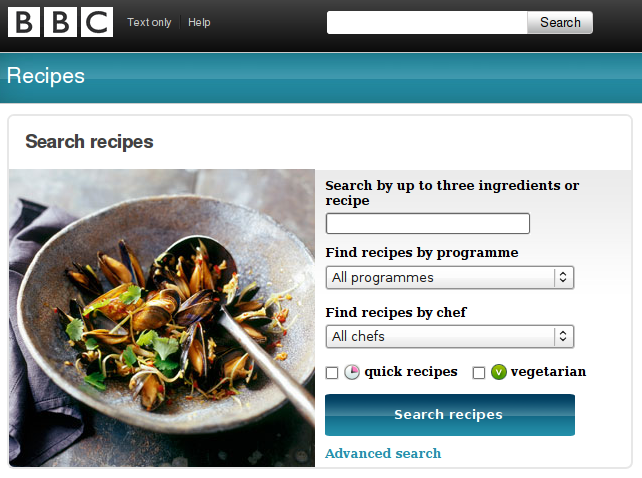
\includegraphics[width=0.9\textwidth]{screenshot_bbc_recipes}
\caption{The BBC Food Recipe Search Page}
\label{fig:bbc_food}
\end{figure}


BBC Recipes (Fig~\ref{fig:bbc_food}) is a web application that allows the user to input up to three ingredients and returns a list of related recipes. 

BBC Recipes has two search options, basic and advanced. The basic search allows the user to input up to three ingredients with the option to find the recipe by television program or by chef. This search also provides the tagging options of quick recipes and vegetarian. However the advanced recipe search includes a wider choice of search preferences such as, the preparation method, cuisine, season and dietary requirements. After looking over the source code it’s very obvious that this web-based application uses an online database using a query language to return recipe results. 

One main advantage about this application is the advanced search option which includes a numerous amount of tag options. This option becomes quite useful when searching through a large database as this kind of search minimizes the results. A good example of this is a search including flour, butter and sugar with the season tag being ‘Christmas’ and the dietary needs tag being ‘nut-free’ returning only 14 recipes. However a search including just the three ingredients returns 400 recipes. 

One flaw that I have noticed with the search is that the search field is a text box which involves text input, this not validating the input until creating the search. The validation matches the input with similar words, for example for ‘flor’ it will return ‘flour’. However when having typo’s like ‘aooples’, instead of ‘apples’ the returned match is ‘allows’. To solve this issue a drop-down menu including the ingredients from the database would perhaps be a better idea.

The design of the website is attractive with a good use of colour and images. However the navigation of the website is slightly tedious, the reason for this being when expanding the actual recipes on the home page the webpage’s content increases and therefore leaving the user to have to scroll through the webpage to view it’s content. 



\subsection{RecipeZaar.com}

\begin{figure}
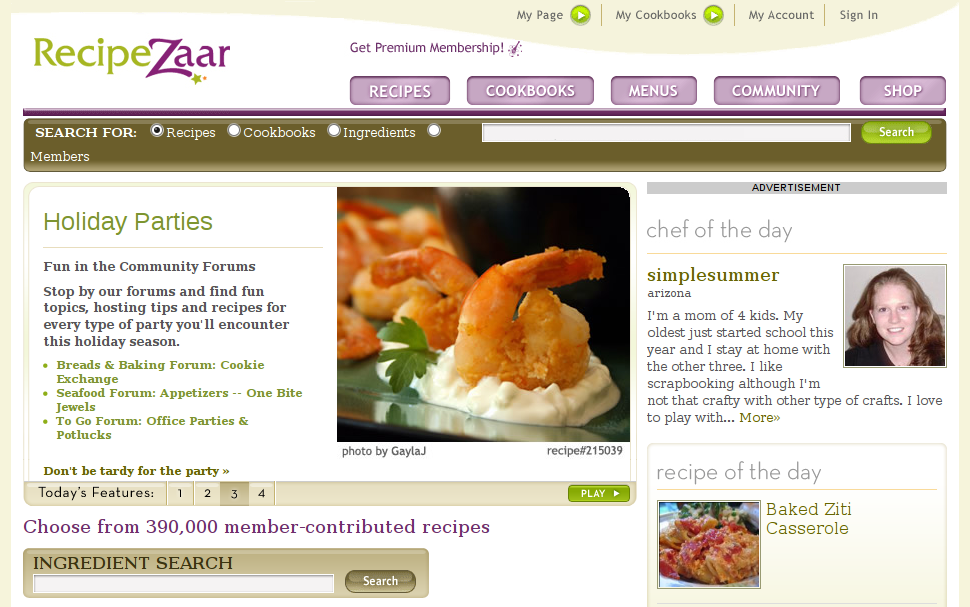
\includegraphics[width=0.9\textwidth]{screenshot_recipezaar}
\caption{The RecipeZaar.com Home Page}
\label{fig:recipezaar}
\end{figure}

Recipezaar (Fig~\ref{fig:recipezaar}) is a website that includes a large database of recipes and user accounts. Recipes are searchable by recipes, cookbooks, ingredients and members. 

The recipe search allows the user to input n number of ingredients. The input method is a text box which includes no validation. If the user inputs ‘flor’ instead of ‘flour’ the search returns nothing. The query used for this search seems to be very basic, the reason for this being if the user inputs ‘flour, sugar, butter, eggs’ for example one of the returned recipes is ‘vegetable casserole’ which doesn’t contain any of the above ingredients. Another example of a recipe is ‘leach family turkey stuffing’ which only contains one of the above ingredients. Because the search isn’t specific and because the website has a large online database the results are too vague.

This website introduces the use of collaborative filtering by including user accounts with the option to upload recipes and rate other recipes. When viewing a member’s recipe theres also the option to send a private message, submit corrections, send the recipe to the users email address or mobile device and create a shopping list. The recipe page also directs the user to other recipes ‘like’ the chosen recipe. The website also has a community webpage with forums for general discussions. 

The design of the website is interactive with a good use of JavaScript. The colour scheme is neutral with a good use of images.



